\documentclass[10pt, conference]{IEEEtran}

\newcommand\textlcsc[1]{\textsc{\MakeLowercase{#1}}}

\usepackage{algorithm}
\usepackage{algorithmicx}
\usepackage{algpseudocode}
\usepackage{balance}

% correct bad hyphenation here
\hyphenation{op-tical net-works semi-conduc-tor}

\usepackage{graphicx}
\usepackage{listings}
\usepackage{color}
\usepackage{soul}  % for \hl{}
\usepackage{amsmath}
%\usepackage{hyperref}
%\usepackage{url,moreverb,xspace}
\usepackage{moreverb,xspace}
\usepackage{booktabs} % For formal tables
\usepackage{multirow}

\definecolor{lightgray}{rgb}{0.95, 0.95, 0.95}
\definecolor{darkgray}{rgb}{0.4, 0.4, 0.4}
%\definecolor{purple}{rgb}{0.65, 0.12, 0.82}
\definecolor{editorGray}{rgb}{0.95, 0.95, 0.95}
\definecolor{editorOcher}{rgb}{1, 0.2, 0} % #FF7F00 -> rgb(239, 169, 0)
\definecolor{editorGreen}{rgb}{0, 0.5, 0} % #007C00 -> rgb(0, 124, 0)
\definecolor{orange}{rgb}{1,0.45,0.13}      
\definecolor{olive}{rgb}{0.17,0.59,0.20}
\definecolor{brown}{rgb}{0.69,0.31,0.31}
\definecolor{purple}{rgb}{0.38,0.18,0.81}
\definecolor{lightblue}{rgb}{0.1,0.30,0.7}
\definecolor{lightred}{rgb}{1,0.4,0.5}


\lstdefinelanguage{javascript}{
  morekeywords={typeof, new, true, false, catch, function, return, null, catch, switch, var, if, in, while, do, else, case, break},
  morecomment=[s]{/*}{*/},
  morecomment=[l]//,
  morestring=[b]",
  morestring=[b]'
}

\lstset{
%     backgroundcolor=\color{backcolour},   
%     keywordstyle=\color{codegreen},
%     numberstyle=\tiny\color{codegray},
%     stringstyle=\color{codepurple},
%     basicstyle={\sffamily},
%     breakatwhitespace=false,         
%     breaklines=true,                 
%     captionpos=t,                    
%     keepspaces=true,                 
%     numbers=left,                    
%     numbersep=5pt,                  
%     showspaces=false,                
%     showstringspaces=false,
%     showtabs=false,                  
%     tabsize=2
  % General design
  backgroundcolor=\color{editorGray},
  basicstyle={\scriptsize\ttfamily},   
  captionpos=b,
  frame=bt,
  % line-numbers
  xleftmargin={0.75cm},
  numbers=left,
  stepnumber=1,
  firstnumber=1,
  numberfirstline=true, 
  % Code design
  identifierstyle=\color{black}\ttfamily,
  keywordstyle=\color{lightblue}\bfseries\ttfamily,
  ndkeywordstyle=\color{editorGreen}\bfseries\ttfamily,
  stringstyle=\color{olive}\ttfamily,
  commentstyle=\color{brown}\ttfamily,
  % Code
  tabsize=2,
  showtabs=false,
  showspaces=false,
  showstringspaces=false,
  extendedchars=true,
  breaklines=true,
  % German umlauts
  literate=%
  {Ö}{{\"O}}1
  {Ä}{{\"A}}1
  {Ü}{{\"U}}1
  {ß}{{\ss}}1
  {ü}{{\"u}}1
  {ä}{{\"a}}1
  {ö}{{\"o}}1    
}

\newcommand{\tool}{\textsc{CanvaSure}\xspace}

\newcommand{\head}[1]{\par\smallskip\noindent\textbf{#1.}}

\begin{document}
%
% paper title
% can use linebreaks \\ within to get better formatting as desired
\title{Web Canvas Testing through Visual Inference}

%\texttt{
\author{\IEEEauthorblockN{Mohammad Bajammal}
\IEEEauthorblockA{University of British Columbia\\
Vancouver, BC, Canada\\
bajammal@ece.ubc.ca}
\and
\IEEEauthorblockN{Ali Mesbah}
\IEEEauthorblockA{University of British Columbia\\
Vancouver, BC, Canada\\
amesbah@ece.ubc.ca}
}
%}}

% conference papers do not typically use \thanks and this command
% is locked out in conference mode. If really needed, such as for
% the acknowledgment of grants, issue a \IEEEoverridecommandlockouts
% after \documentclass

% for over three affiliations, or if they all won't fit within the width
% of the page, use this alternative format:
% 
%\author{\IEEEauthorblockN{Michael Shell\IEEEauthorrefmark{1},
%Homer Simpson\IEEEauthorrefmark{2},
%James Kirk\IEEEauthorrefmark{3}, 
%Montgomery Scott\IEEEauthorrefmark{3} and
%Eldon Tyrell\IEEEauthorrefmark{4}}
%\IEEEauthorblockA{\IEEEauthorrefmark{1}School of Electrical and Computer Engineering\\
%Georgia Institute of Technology,
%Atlanta, Georgia 30332--0250\\ Email: see http://www.michaelshell.org/contact.html}
%\IEEEauthorblockA{\IEEEauthorrefmark{2}Twentieth Century Fox, Springfield, USA\\
%Email: homer@thesimpsons.com}
%\IEEEauthorblockA{\IEEEauthorrefmark{3}Starfleet Academy, San Francisco, California 96678-2391\\
%Telephone: (800) 555--1212, Fax: (888) 555--1212}
%\IEEEauthorblockA{\IEEEauthorrefmark{4}Tyrell Inc., 123 Replicant Street, Los Angeles, California 90210--4321}}

% use for special paper notices
%\IEEEspecialpapernotice{(Invited Paper)}

% make the title area
\maketitle

\begin{abstract}
\begin{abstract}

Filling web forms is a common online activity. 
Web forms are made accessible to users with disabilities 
by conveying their content through specific DOM labeling 
markups. The absence of these markups is one of the most 
common accessibility errors. However, there is currently 
little to no work in terms of having an automated analysis 
process that allows inferring the labeling markups in order 
to automatically make forms accessible for users with disabilities. 
In this paper, we propose a web form analysis approach that 
infers labels by first constructing different types of 
visual cues from a form, then optimizing the combination of 
various cues and form fields, and finally augmenting the DOM 
to incorporate the required labeling markup. We evaluate 
our approach on real-world subjects and assess the accuracy 
of labeling inference, the safety of the DOM augmentation, 
as well as the labeling performance. The results show an 
average F1-measure of 88.4\% for label inference, and an 
average run-time of around 1.6 seconds.

\end{abstract}

\keywords{web forms, accessibility errors, 
accessibility repair, visual analysis}

\end{abstract}

\begin{IEEEkeywords}
web canvas elements; web testing; DOM augmentation; image analysis

\end{IEEEkeywords}

% For peer review papers, you can put extra information on the cover
% page as needed:
% \ifCLASSOPTIONpeerreview
% \begin{center} \bfseries EDICS Category: 3-BBND \end{center}
% \fi
%
% For peerreview papers, this IEEEtran command inserts a page break and
% creates the second title. It will be ignored for other modes.
\IEEEpeerreviewmaketitle

% !TEX root =  manuscript.tex
%\IEEEraisesectionheading{
	\section{Introduction}\label{sec:introduction}
%}


% \IEEEPARstart{S}{oftware} engineering (SE) is the application of
% a systematic, disciplined, quantifiable approach to
% the development, operation, and maintenance of 
% software~\cite{IEEEComputerSociety:2014:GSE:2616205}. 
%\IEEEPARstart{A}{ll} 
All areas of the software engineering (SE) lifecycle, 
such as requirements, design, development, and testing, 
often have the ultimate goal of contributing to a
fundamental product of software engineering: the source code.
Accordingly, a wide range of software engineering activities have
typically revolved around the source code,
whether to improve its quality, reliability, maintainability,
 or increase developers' productivity.
A relatively more recent, and scarcely explored, 
alternative is the adoption of a 
\emph{visual analysis} perspective.
This approach aims to extract, analyze, or process visual aspects
pertaining to the software, often using computer vision techniques. 
The objective is still focused on solving a software engineering problem, 
but is achieved via analyzing visual aspects of the software instead of relying 
exclusively on the source code.
As an example, a typical visual analysis  
might involve comparing a couple of screenshot images in order  
to compare or analyze two graphical user interfaces (GUI)
for testing purposes. 

Visual analysis techniques have yielded promising results 
in developing robust and accurate solutions
for various tasks.
For instance, they have been successfully adopted
to improve regression testing of GUIs
~\cite{Chang-2010-CHI, Alegroth-2013-ICST, Lin-2014-TSE},
to identify cross-browser incompatibilities in web pages
~\cite{Semenenko-2013-ICSM,Choudhary-2013-ICSE,Selay-2014-DICTA}, to 
perform bug detection and automated program repair~\cite{Mahajan-2014-ASE, Stocco-2018-FSE}, 
or to simplify software requirements modelling
~\cite{Li-2010-CHI, Scharf-2013-ICSE}.

In this chapter, we survey the literature on 
the use of visual analysis in performing 
software engineering tasks. 
Our work highlights visual analysis techniques and perspectives
of addressing research topics in software engineering,
what benefits they may provide compared to existing approaches,
and what limitations they might bear.
We believe this can be helpful in
providing a distilled and concise overview of 
visual approaches in software engineering, 
building a concrete understanding of the 
advances made, and synthesizing insights  
regarding future directions for the research community. 
We conducted the survey by formulating a number of
research questions to fulfill the goal of the study;
we then proceeded by systematically collecting
a pool of publications, and applied a number of
inclusion and exclusion criteria.
Subsequently, we analyzed and synthesized the collected papers
by taking into account a number of dimensions,
such as what area of software engineering (e.g., testing, maintenance)
they brought benefit to, 
what specific task is being addressed (e.g., regression testing),
what specific computer vision (CV) techniques have been used,
and what is the rationale for their adoption.


%\newpage
\section{Motivating Example}\label{sec:motivating}

\begin{figure}[t]
    \centering
    \includegraphics[trim={0.1cm 0.1cm 0.1cm 0.1cm},clip,width=0.58\textwidth,height=0.36\textheight]{testability/figures/motivating-example-new.png}
    \caption{An example canvas-based application. When the button is clicked, the plot is drawn dynamically (on the client side) using the canvas element.}
    \label{fig:motivating-example-1}
\end{figure}


Figure~\ref{fig:motivating-example-1} shows an example web application that uses canvas elements.
A bar chart is drawn in the canvas when the user clicks the button.
The corresponding JavaScript code is shown in Listing~\ref{lst:motivating-example-1}.
This example illustrates the dynamic nature of canvas-based web applications.
The data is plotted dynamically, on-the-fly, on the client side as opposed to the latency involved in sending the data to be plotted at a server that replies back with an image of the generated bar chart.
This dynamic nature makes canvas elements useful in interactive and high-performance visualizations and graphics.

Listing~\ref{lst:motivating-example-1} shows a snippet of how the setup and manipulation of canvas elements is done exclusively through the Canvas JavaScript API~\cite{w3c_canvas_standard}.
The canvas API provides functionality to draw lines, circles, rectangles, etc.
These can then be combined and dynamically added to the canvas element in order to draw more complex and interactive drawings.
Lines 6 to 11 show a snippet of how the canvas API is used to draw a rectangle on the chart.
A call is made to the \verb|fillRect()| function from the canvas API with parameters specifying the rectangle.
This allows dynamic creation of shapes on the canvas.

However, the HTML canvas element itself (Listing~\ref{lst:motivating-example-1}, lines 17-21)  remains empty throughout the entire usage of the application.
The execution of various canvas API functions does not change or update the contents of the canvas element tag.
\hl{This is because, as required by the official W3C standard~\mbox{\cite{w3c_canvas_standard}} of canvas elements, the canvas has no DOM representation. That is, the DOM subtree under a canvas node remains empty, and therefore its state remains unobservable. 
Instead, the canvas API functions are required to draw \mbox{\emph{directly}} to the raw monitor pixels buffer without the costly task of maintaining a DOM representation. This direct drawing allows canvas elements to achieve high-speed performance in order to enable dynamic and highly-interactive applications. }

Unfortunately, this DOM-free nature that enables the high-speed of canvas elements is also the reason why they are more difficult to test.
At any point during the execution of the application, the state of the canvas remains unobservable.
While one might conceptually think of gathering state information by tracking the call stack of the API calls, this would not be applicable to an exclusively visual API such as that of the canvas.
This is because the actual visual rendered canvas does not directly correspond to the calls made to its API.
For instance, calls could mistakenly visually override one another, or they might call the API with unintended arguments, resulting in a wrong visual result. 
A thousand canvas API calls (for example, draw the rectangle in the example, \emph{one point} at a time) can produce the same resulting visual state as one canvas call (a single call to \verb|fillRect|).
Consequently, we can see that it is difficult to assess what state is the canvas in at any given moment which makes it difficult to test canvas elements.

\hl{In this chapter, we propose an approach that makes canvas elements testable. That is, the goal is to 
provide developers with the fundamental capability of observing the canvas state and making assertions on it. However, the aim is not to provide a complete testing solution, but rather to enable the 
testing process itself, thereby improving testability. This approach visually analyzes the canvas screenshot, then creates a DOM tree representing the visual state of the canvas.
This makes it possible to test the canvas element using common DOM-testing techniques.
Finally, the developers would write their own tests, or could optionally use the automatically generated tests to check the visual objects of the canvas and their properties.}


\begin{lstlisting}[language={javascript},
float=tbp,
aboveskip=1.4em,
caption=JavaScript and HTML snippet of the canvas drawing in Figure~\ref{fig:motivating-example-1}., 
label={lst:motivating-example-1}]

function onButtonClick() {
	var canvas = document.getElementById("canvasBarChart
").getContext("2d");
	...
	canvas.beginPath();
	...
	// Example: this would draw one of the
	// rectangles in the bar chart.
	canvas.fillRect(leftCoordinate, topCoordinate,
					width, height);
	...
}


// The HTML portion of the app
<canvas id="canvasBarChart">
	// This tag remains empty throughout the usage of
	// the app, due to the lack of DOM representation
	// for canvas elements.
</canvas>

\end{lstlisting}
% !TEX root =  paper.tex

\section{Proposed Approach}\label{sec:approach}

\begin{figure}[t]
    \centering
    \includegraphics[trim={0.0cm 0.0cm 0.0cm 0.0cm},clip,height=7.9cm,width=0.62\textwidth]{testability/figures/canvasure-overview-figure.pdf}
    \caption{Overview of the proposed approach.}
    \label{fig:approach-overview-1}
\end{figure}

The approach starts by automatically opening the webpage containing canvas elements in an instrumented browser.
It focuses on canvas elements only and is therefore agnostic of the rest of the web application's page.
Therefore, it can analyze canvas elements contained in a larger webpage or canvas applications that are solely composed of a single canvas element.

\subsection{Overview}
Figure \ref{fig:approach-overview-1} depicts an overview of the main steps of the proposed approach.
For each canvas element on the page, a screenshot is captured and visually analyzed.
The visual analysis begins by performing a visual identification of objects on the canvas.
Our object identification is capable of identifying common geometrical shapes supported by the canvas API, such as lines, circles, and rectangles, as well as generic arbitrary shapes.
Next, the approach infers the visual properties such as color, size, and location, for each of the detected visual objects.
A list of all supported properties is shown in Table \ref{tbl:info-provided-by-approach}.
Subsequently, the approach builds a hierarchy information of the visual objects contained in the canvas.
This hierarchy information includes parent-child relations between objects, indicating which objects (if any) are contained inside other objects.
The hierarchy also includes z-order information, which indicates front-to-back arrangement of overlapping objects.

All the information extracted through the previous steps is then represented as an augmented DOM inside the canvas element.
The testing of the canvas is performed by generating assertions from the augmented canvas DOM.
We now describe each of these steps in detail in the following subsections.
 

\subsection{Visual Object Identification}
\label{subsec:viz-identification}
The objective of this stage is to detect and identify objects that are present on a canvas element.
We define an object to be present on the canvas if it is rendered and visible in the current screenshot of the canvas.
However, the approach does not require an object to be fully visible; occlusions and overlaps of multiple objects are allowed.
We apply a number of transformations on a copy of the original canvas image, $\mathbf{C_T}$, in this stage.

\head{Color contrast adjustment}
The goal of this first step is to perform a form of color contrast adjustment of the canvas screenshot.
This is performed in order to enable our analysis to \emph{see} objects more clearly. 

The analysis performs the color contrast adjustment through a \emph{color space conversion} of the canvas screenshot,  $\mathbf{C_T}$.
A color space conversion changes the representation of the colors of the pixels from one representation system to an alternative representation. 

We first need to select a suitable conversion method since several methods exist.
To that end, we perform an empirical examination of the eight most common conversion methods \cite{tooms2016colour}, namely HSV, L*a*b*, L*u*v*, CIE-RGB, XYZ, YUV, YIG, YPbPr, and YCbCr.
Each of these is simply a mathematical formula \cite{tooms2016colour} that changes pixels from one color representation to another. 

We empirically evaluate these conversions on a random set of 20 canvas elements.\footnote{http://corehtml5canvas.com} The results of this empirical examination are shown in Figure \ref{fig:param-est-colorspace}.
The figure shows how much contrast there is in the canvas image when using the different color conversions. The contrast is measured using 
the variance in pixel values. Higher values in the figure indicate  more contrast. Based on the results shown in the figure, the YCbCr conversion yields the best color contrast.
YCbCr will therefore be our choice for the color space that the canvas will be converted to.
Therefore, the algorithm creates a new image, $\mathbf{\bar{C}_T}$, which represents the canvas screenshot in YCbCr.
An example of the outcome of this step is shown in Figure \ref{fig:stages-examples}-a for a part of the motivating example.


\head{Detecting object boundaries}
The goal of this step is to detect the boundary of each object in the canvas.
This is performed in order to allow the analysis to roughly estimate where the objects are in the canvas image; this boundary information is used later to identify objects and their properties.

In order to detect these boundaries, we calculate the image gradient \cite{fernandez2012advanced}.
The image gradient is a mathematical processing applied on the canvas image to extract edges, which are the parts of the canvas where there is a transition from one object to another; for example, a boundary between an object and its background.

First, we need to select a suitable method to calculate the image gradient since several methods exist.
In order to be able to compute more accurate gradients for various canvas object shapes, we use the Scharr method \cite{scharr2000optimal}.
We make this choice because this method has been shown \cite{kroon2009numerical} to yield good results for smooth and curved objects in addition to angled objects.
 This would therefore be suitable for processing objects found on canvas elements.
  We compute the image gradient on $\mathbf{\bar{C}_T}$, and call it $\nabla \mathbf{\bar{C}_T}$.

Next, the analysis performs a binary transformation and converts each pixel in $\nabla \mathbf{\bar{C}_T}$ into either 0 or 1.
 A value of 1 represents a pixel that is on the object boundary, and a value of 0 means otherwise.
  The processed canvas image is called $(\nabla \mathbf{\bar{C}_T})^B$. 
To compute $(\nabla \mathbf{\bar{C}_T})^B$, we need to perform thresholding on the image, i.e., the reduction of a graylevel image to a binary image. 
We choose a machine learning clustering approach called Otsu thresholding from the computer vision literature, to perform this thresholding.
 Otsu's method is clustering-based and has been shown \cite{sezgin2004survey} to yield high performance. The outcome of this step is depicted in Figure \ref{fig:stages-examples}-b for the motivating example. 


\head{Separating objects}
So far, we have a collection of boundaries, but we do not know which group of boundaries belong together as part of the same object.
The goal of this step is to separate the different boundaries detected in the last step. 

\begin{figure}[t]
    \centering
    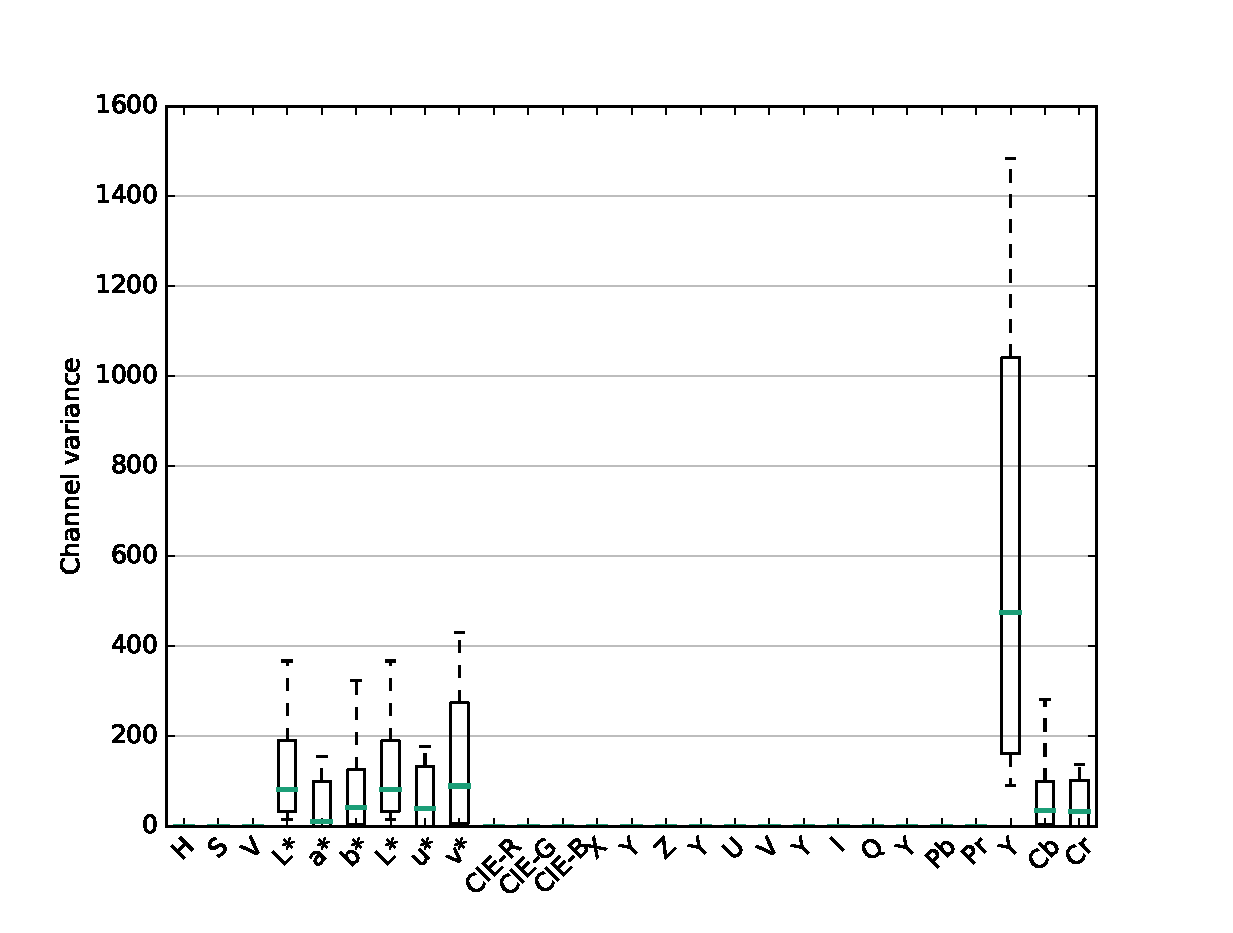
\includegraphics[trim={0.3cm 0.3cm 0.3cm 0.3cm},clip,height=0.35\textheight, width=0.74\textwidth]{testability/figures/colorspace-parameter.eps}
    \caption{Parameter estimation for the color contrast adjustment step of the algorithm. Choosing the YCbCr color representation yields best contrast adjustment for the canvas screenshot. Higher values are better. }
    \label{fig:param-est-colorspace}
\end{figure}



First, our analysis goes through the list of all detected boundaries. For each boundary, the algorithm walks on the boundary, step by step, and examines which other boundaries are connected to it. At the end of this process, we have a group of disjoint boundaries $\mathbf{B}_i$:
%\begin{align}
\begin{equation}
\label{eqn:approach-regions}
(\nabla \mathbf{\bar{C}_T})^B = \bigcup \mathbf{B}_i \,\, : \,\, \bigcap \mathbf{B}_i \equiv \O
\end{equation}
%\end{align}	
where $\mathbf{B}_i$ is a set containing the boundary pixels of the $i^{th}$ detected object in the canvas. The equation shows that each boundary $\mathbf{B}_i$ is separate from other boundaries, $\mathbf{B}_{j\neq i}$.

The algorithm then proceeds by computing the \emph{Euler number} \cite{sossa1996computation} for each boundary $\mathbf{B}_i$. The Euler number is a metric that shows whether a boundary has branches, or is a continuous boundary. For example, geometric shapes such as rectangles or circles have boundaries that continuously surround the shape without branching. On the other hand, two rectangles sharing an edge will have a branch in their boundary.

Next, the algorithm uses the Euler number $\mathcal{E}$ that was just computed in order to check for branching in a boundary. A value of $\mathcal{E} = 0$ indicates that the boundary is one continuous shape without branching. For this case, the algorithm saves the boundary as is without further modifications. On the other hand, a value of $\mathcal{E} < 0$ indicates that a boundary has branching. In this case, the algorithm breaks down the original boundary and creates new boundaries for each branching. We note that this will not cause 
any unnecessary or excessive fragmentation of the structure, 
because the fragmentation only occurs when the boundary branches, 
and no branching occurs for continuous (i.e., unbranched) segments 
of the object.  

At this stage, the analysis has extracted a set of boundaries $\mathbf{B}_i$ from the canvas image that are separate from each other and non-intersecting.  
An example of the outcome of this step is shown in Figure \ref{fig:stages-examples}-c.

\head{Extracting segments on boundaries}
The purpose of this step is to help identify the type of each object (e.g., rectangle, circle, arbitrary shapes, etc) based on extracted segments from its boundary. To this end, we take the object boundaries detected so far and break them into smaller line segments.  Objects that are curved and smooth, such as circles or generic shapes, are still represented by linear segments too, but as minuscule lines at a zoomed-in scale. While more complicated computer graphics models might be used (e.g., curves, polynomials), we opted 
for linear segments to simplify the analysis and make it faster. 

Following the detection of all boundaries $\mathbf{B}_i$, 
we need to understand what the \emph{identity} of each boundary is. 
This is because, at this stage, we only have a collection of boundaries but do not know what shapes do they represent, or 
what their properties are (e.g., dimensions, colors). 
The first step towards gaining this information is to segment these boundaries or break them down into smaller sections. 
Accordingly, the analysis proceeds by populating each boundary with a random set of probabilistic Hough segments from the computer vision literature \cite{matas2000robust}. These segments are small linear portions of the boundary of each region. This approach has been shown \cite{kiryati2000randomized} to produce robust extraction of boundary segments. In essence, this step performs rough clustering of boundary coordinates and groups neighboring points into a set of small segments.

The generated probabilistic segments are, however, often redundant duplicates, overlapping, and/or intersecting. 
This is because the aforementioned Hough segmentation process is stochastic in nature and while it is robust in most situations, its stochastic nature does cause to generate false positives. 
This presents a challenge in terms of identifying which segment is a true linear segment and which is redundant. 
As such, the set of all generated segments does not have a direct 1-to-1 correspondence to linear segments on the boundary.

We address this by performing a post-processing of the generated segments. Post-processing starts by creating an \emph{R-tree} index. An R-tree~\cite{hadjieleftheriou2008r} is a database structure that allows storing, querying, and retrieving data that is spatial in nature (e.g., locations, point sets). Our set of segments is also an example of such spatial data. Therefore, we insert the segments into an R-tree index in order to efficiently perform spatial queries such as finding intersecting segments or neighbors.
 
Accordingly, two sets of operations are performed on the R-tree index. The first operation consists of iterating through each line segment in the index and then querying the existence of other segments with full or partial spatial intersection. The second operation also iterates through each line segment in the index, but queries the existence of neighbouring segments instead of intersections.

For the first R-tree operation, the result of each iteration is a set of segments that are fully or partially intersecting. The algorithm then performs a pair-wise iteration over the intersecting subset. For a pair of line segments that are parallel, the algorithm removes the smaller segment if it is fully enclosed in the larger segment. Otherwise, in cases where the rectangles (which represent the bounding boxes of objects) are partially overlapping, the two parallel segments are merged into one new line segment, and then removed from the set.

\begin{figure}%[b]
    \centering
    \includegraphics[trim={0.0cm 0.0cm 0.0cm 0.0cm},clip,height=7.5cm,width=0.35\textwidth]{testability/figures/stages-illustration.png}
    \caption{Illustration of the general stages involved in the visual identification of canvas objects. Best viewed on a color monitor. }
    \label{fig:stages-examples}
\end{figure}

For the second R-tree operation, the result of each iteration is a subset of segments that are neighbours of each other. The algorithm forms this subset by querying the R-tree index for the 4 spatial neighbours, one neighbour in each direction, around the query rectangle. The algorithm then performs a pair-wise iteration over the subset. Pairs that are both collinear and parallel are then merged into one new segment, and the forming segments are dropped from the set. Other pairs are left in the set as is.

%\begin{table*}[tb]
\begin{sidewaystable}
\setlength{\tabcolsep}{6pt}
\renewcommand{\arraystretch}{0.9}
\centering
\caption{List of the information that is visually inferred from the screenshots of web canvas elements}
%\begin{tabular}{lccc}
\begin{tabular*}{0.99\textwidth}{l @{\extracolsep{\fill}} ll}
\toprule
\textbf{Visual object identity} &  \textbf{Visual properties}  &  \textbf{Hierarchical structure} \\

\midrule
lines, triangles, rectangles,  &  - centroid: geometric center point of objects & - z-order: relative order of objects \\

squares, circles, & - size: & in the z-direction (i.e. behind or \\

generic shapes (polygons) & \, \, \, - width and height: for rectangles and squares & in front of other objects) \\

 & \, \, \, - diameter: for circles &  \\ 
 
* Note: our approach allows  & - color (HTML hex values) & - Parent-child relation: which \\

multiple overlapping, partially  & - orientation: number of degrees of rotation from horizon & objects are contained inside  \\

visible, or nested combinations & - point-set: the set of points representing generic shapes (polygons) & other objects. \\

of these objects. & & \\ 
 
\bottomrule
%\end{tabular}
\end{tabular*}
\label{tbl:info-provided-by-approach}
%\end{table*} 
\end{sidewaystable}


At this point, we have constructed a final set of line segments for each boundary. The analysis is ready to identify the shape type (e.g., lines, rectangles) of each object. An object whose set of segments has a cardinality of 1 is reported as belonging to the `line' type. Similarly, a set of three connected lines are triangles, and four lines are rectangles. For other objects, the analysis first performs an ellipse fitting to cover the object. Then, the relation between the major and minor axes of the ellipse is computed. If these axes are equal, then the detected shape is identified as a circle if the object's set of line segments has a cardinality of more than 4 (i.e. more than a rectangle) and its area is \emph{solid}. These set of conditions define what a circle is exactly. This is because a  region is defined as \emph{solid} when the the area of that region is identical to the area of the convex hull of the same region. On the other hand, when the region is not solid, the object is identified as a polygon.
Table \ref{tbl:info-provided-by-approach} lists the different object types recognizable by our approach. These types are the same types of objects provided by the canvas API. We note that our approach does not require any training dataset like machine learning approaches, because the attributes and identities of various shapes can be more precisely and robustly captured using mathematical ratios such as the process conducted in this step.
 
\subsection{Visual Properties Measurement}
\label{subsec:viz-props}

At this stage, our technique measures the visual properties of the objects detected in the previous section. These properties are extracted from the original canvas screenshot and include parameters such as location, size, and color. Table \ref{tbl:info-provided-by-approach} shows a list of the visual properties that are measured by the technique for the detected visual objects. This subsection describes the process by which we measure these properties.

\head{Object position} First, the technique calculates the centroid of each detected object. This is done by computing the arithmetic mean of all coordinates in the object. The centroid would therefore represent the point that minimizes the average Euclidean distance between itself and other coordinates in the object.

\head{Color} Next, for all coordinates in the object, the analysis computes the median pixel vector. This is performed to remove outliers that might be present due to small protrusions in the detected region. This vector is then assigned to the color property of the detected object.

\head{Size and orientation}
Subsequently, the analysis performs an ellipse fitting to the region of the object. The ellipse is centred on the centroid, and its axes are fitted so that the ellipse covers the entire object. By the end of this process, an ellipse is generated for each detected object, with each ellipse having a centre, a major axis, and a minor axis. The analysis then extracts a number of visual properties based on the fitted ellipse. First, if the shape is a rectangle, the ellipse axes determine the width and height because the ellipse's major and minor axes would align with the rectangle's axes. If the shape is a circle, then ellipse axes determine the diameter. Next, an orientation is assigned to the object. This orientation is computed as the angle between the major axis of the ellipse and the positive horizontal axis. This represents how much the object is rotated. 


\head{Point set}
Finally, the analysis extracts a representative point set for each object. This point set lists the coordinates necessary to reconstruct the object. This set is only generated for triangles and generic shapes (polygons), since other object categories are fully identified using their other measured properties, as shown in Table \ref{tbl:info-provided-by-approach}. 
In order to generate this representative point set, the analysis takes as input the coordinates of the object boundary and then proceeds to apply the \emph{Harris} operator for the computer vision literature \cite{ryu2011formula}, which is a mathematical transformation that detects points of intersections in boundaries. This process extracts points with more than one directions of lines coming in/out of it, which yields points where linear segments intersect. 
 
\subsection{Hierarchical Structure Inference}

For each detected canvas object, the analysis then performs a sequence of operations on the canvas screenshot that we have processed so far in order to infer any hierarchical information. We define hierarchical information as the information pertaining to the relative spatial relations between overlapping or nested objects. Objects that are not overlapping or nested have no hierarchical information.

More specifically, the hierarchical information of an object has two parts: the z-order and the parent-child relations. 
The z-order determines the relative arrangement of overlapping objects along the z-axis (i.e., front to back arrangement). While the width of the screen is represented with an x axis and the height of the screen represented by a y axis, the z-axis is perpendicular to the xy screen plane and points towards the user. That is, it determines which objects are closer to the viewer and away from the screen, and which are away from the viewer into the screen. 

The second part of hierarchical information is the parent-child relations.
This hierarchical information examines nested objects and determines which are children objects and which objects are their parents.
We define object A to be a child of object B if object A is entirely visually contained inside object B.
Equivalently, object B is a a parent of object A if it entirely contains it.
Objects that are not fully contained in other objects (for example, in cases of partial overlaps) are siblings, and do not have a parent-child relation.

The analysis starts the inference process by creating two directed acyclic graphs for the detected objects.
The first graph, $\mathbf{P}$, captures parent-child information.
The second graph, $\mathbf{Z}$, contains z-order information.
Every object is initialized as a degree zero vertex on the graphs.
Subsequently, the analysis creates an R-tree index. Each item in the index is a 2-tuple of a detected object and its minimum bounding rectangle. 

The analysis then iterates over the collection of detected objects.
For each object, the analysis performs a spatial query on the R-tree to determine the leaves that are intersecting with the object.
This results in one of three possible scenarios.
The first is when the R-tree returns no intersections with the object.
The second is when the intersecting object has its minimal rectangle fully inside the query object.
The third case is when the intersecting rectangles are partially overlapping.

For the first case, the minimal rectangles of the tree leaves are non-intersecting.
This query result indicates that there are no overlapping or nested objects with the current object.
As such, the object has no defined hierarchical information.
The $\mathbf{P}$ and $\mathbf{Z}$ graphs are therefore not updated, and the corresponding vertices of the object remain in their initial state of zero degree.

For the second case, the query indicates that one or more objects are fully contained inside the query object.
Therefore, this constitutes a parent-child relation.
Accordingly, we update both graphs $\mathbf{P}$ and $\mathbf{Z}$.
The update to $\mathbf{P}$ is a new directed edge from the child to the parent.
Similarly, the update to $\mathbf{P}$ is also a directed edge from the child to the parent.

Finally, for the last case, the query returns a partial overlap of the minimal rectangles.
As such, this case would not constitute a parent-child relation.
However, it is still possible for this case to have z-order relations.
Accordingly, the analysis proceeds to detect the presence of a z-order relation.
First, the analysis generates the concave parts of the region.
These parts are the subtraction of the convex hull of the region from the original region.
Next, the analysis performs an element-wise logical XOR between concave parts of the object and the objects with the partially overlapping minimal rectangles.
If the result of the operation is a non-zero region, then a z-order relation exists.
The analysis proceeds by creating a directed edge in $\mathbf{Z}$ from the object with the concave parts to the object that is resulting from the R-tree query.


\subsection{Testing through DOM Augmentation}
\label{subsec:testing-using-dom}
At this stage, the analysis has concluded the process of building information about the identity, properties, and hierarchical structure of the objects on the canvas. The analysis proceeds by casting this information into a DOM tree and augmenting it to the original canvas element.

\head{DOM Augmentation}
First, the analysis creates a DOM node for each detected object on the canvas. The tag name of the node matches the identity of the object. For example, an object that has been identified as a triangle is represented as \verb|<triangle>|, generic shapes (polygons) as \verb|<polygon>| and so on. 

Next, for each node in the DOM, the analysis inserts all the detected attributes pertaining to the identified object (see Table \ref{tbl:info-provided-by-approach} for a full list of attributes). For example, a \verb|diameter| attribute is added to each \verb|<circle>| node.

Finally, the analysis then proceeds by arranging the nodes of the DOM according to the inferred hierarchical information. We recall that the hierarchical information consisted of two parts: the parent-child relations contained in the $\mathbf{P}$ graph, and the z-order relations contained in the $\mathbf{Z}$. For the parent-child relation, the analysis re-orders the nodes of the DOM as to make child nodes in the DOM correspond to child objects on the canvas (as described in the hierarchical structure extraction section). The analysis then adds a \verb|z-order| attribute to each node. A z-order of zero indicates a front-most object, and elements further back have increasing negative values.

\lstdefinelanguage{HTML5}{
	language=html,
	alsoletter={-,=},
	otherkeywords={
		% HTML tags
		<html>, <head>, <title>, </title>, <meta, />, </head>, <body>,
		<canvas, </canvas>, <rectangle, </rectangle>, <triangle, </triangle>, <script>, </script>, </body>, </html>, <!, html>, <style>, </style>, ><
	},  
	ndkeywords={
		% General
		=,
		% HTML attributes
		charset=, id=, center=, color=, z-order=, point-a=, point-b=, point-c=,width=, height=,
		% CSS properties
		border:, transform:, -moz-transform:, transition-duration:, transition-property:, transition-timing-function:, z-order=
	},
	morecomment=[s]{<!--}{-->},
	tag=[s]
}

\begin{lstlisting}[language=HTML5,float=*,caption={The visually inferred augmented DOM for the canvas element of the motivating example (Figure \ref{fig:motivating-example-1} and Listing \ref{lst:motivating-example-1})}, label={lst:augmented-DOM-result}]
	<canvas id="canvasBarChart">
	
	<rectangle center="(191,43)" width="86" height="295" z-order="-1" color="#673C8C">
	<triangle center="(107,43)" point-a="(93,43)" point-b="(114,33)" point-c="(114,55)" z-order="0" color="#41A74D"/>
	</rectangle>
	
	<rectangle center="(166,264)" width="87" height="355" z-order="-1" color="#673B8C">
	<triangle center="(57,264)" point-a="(43,265)" point-b="(64,254)" point-c="(64,276)" z-order="0" color="#41A74D"/>
	</rectangle>
	
	... the rest of the generated DOM ...
	</canvas>
\end{lstlisting}

At this stage, the analysis has finished constructing an augmented DOM tree for the canvas element. An example is shown in Listing \ref{lst:augmented-DOM-result} representing the generated augmented DOM corresponding to the motivating example. As shown in lines 4 and 8 of the listing, a triangle node is located inside a rectangle node in the DOM. This corresponds to the state of the original canvas in Figure \ref{fig:motivating-example-1}, where one can see that a triangle is visually located inside a rectangle.


\head{Testing process}
The proposed canvas DOM augmentation approach was designed to extend and enable the use of DOM testing techniques with canvas elements. As such, it can be used in any testing process that is based on the DOM. For example, through browser automation using Selenium, a test can be written to navigate to a page, click a few buttons, and then finally, through the proposed augmentation approach, assert that the canvas has a vertical red rectangle, for instance. This is similar to the common task performed in DOM tests when the presence of a certain element, say a \verb|<div>| with a certain id, is asserted. 

The inferred augmented DOM is then used to test the canvas element in one of two ways. In the first testing approach, a list of assertions can be automatically generated by default to assert the presence of all nodes of the DOM and their attributes and hierarchy, as shown in Listing \ref{lst:generated-tests}. The generated assertions are broken down into three types of assertions that correspond to the information inferred from the canvas: (a) assertions on the identity of objects, (b) assertions on the properties of objects, and (c) assertions on the hierarchy of objects. The reason for separating assertions into three different layers is twofold. First, this enables pinpointing the cause of assertion failures, as opposed to writing one assertion that asserts the state of the entire canvas as a whole. Second, this strategy gives the user a flexible way of choosing which aspect of the canvas to test. For instance, the user can indicate that they are only interested in testing the presence of objects on the canvas, regardless of position or color. Of course, the user can keep the default option where all attributes are tested. Therefore, instead of just simply reporting that a test has failed, the approach, for example, can report that the test has failed because a triangle was absent or has changed color in the canvas.

Alternatively, in the second testing approach, the augmented DOM can be used in a case where a tester would write specific tests to assert the existence of particular objects, properties, or certain hierarchies of interest. %This would then only test the assertions specified by the tester. 
This use case would, therefore, be more appropriate for scenarios such as test-driven development, for instance.
However, we emphasize that the goal of the proposed approach 
is to provide developers with the \emph{ability} to test canvas elements, since they are not testable at the moment. That goal is the priority, more so than providing a complete end to end testing 
solution that would cover all the possible ways or markups 
that developers would prefer to write their tests in. 

     \begin{lstlisting}[language=Java, float=*, caption={The automatically generated test assertions for the canvas element of the motivating example (Figure \ref{fig:motivating-example-1} and Listing \ref{lst:motivating-example-1})}, label={lst:generated-tests}]
// High-level test: testing the identity of objects in the canvas
 assertTrue("'canvasBarChart' should contain 5 triangles",
   webDriver.findElements(By.xpath("//canvas[@id='canvasBarChart']//triangle")).size() == 5);

 assertTrue("'canvasBarChart' should contain 5 rectangles",
   webDriver.findElements(By.xpath("//canvas[@id='canvasBarChart']//rectangle")).size() == 5);
   // ...

// More detailed test: testing the locations of objects in the canvas
 assertNotNull("'canvasBarChart' should contain a triangle at (107,43)",
   webDriver.findElement(By.xpath("//canvas[@id='canvasBarChart']//triangle[@center='(107,43)']")));
	// ...

// More detailed test: testing the size of objects in the canvas
 assertNotNull("'canvasBarChart' should contain a rectangle with width=86 and height=295",
   webDriver.findElement(By.xpath("//canvas[@id='canvasBarChart']//rectangle[@width='86' and @height='295']")));
	// ...

// ... Tests for other properties (z-order, color, etc)
     \end{lstlisting}
	

\header{Implementation}
We implemented our canvas visual inference approach in a tool called \tool\cite{canvasure}. \tool is implemented in Python 3. We use the numpy~\cite{walt2011numpy} library to import basic mathematical and numerical functions, and use the scipy~\cite{jones2014scipy} library for matrix computations on the screenshots. We use the Selenium web driver to run and instrument web applications and extract canvas elements.



\section{Evaluation}

\label{sec:evaluation}
We conducted qualitative and quantitative studies  
to answer the following research questions:

\begin{enumerate}[label=\textbf{RQ\arabic*},leftmargin=*]
	\item How accurate is the labeling associations inference? 

	\item How safe is the labeling markup repair process?
	
	\item How scalable is the performance with the size of 
	real-world web forms? Is it suitable for real-time usage?
\end{enumerate}

In the following subsections, we discuss the details of the experiments that 
we designed to answer each research question, together with the results and discussions.

\subsection{RQ1: Inference Accuracy}\label{subsec:rq1}
In this question, the objective is to assess how accurate 
is the inference of the labeling associations in a given web form. 
We recall that, as per the ARIA standard, a web form is accessible 
if it has markup that correctly captures the labels on the form. 
Accordingly, the most important evaluation question is to 
assess how accurate are the inferred form labels. 

We evaluated this research question as follows. 
First, we collected 30 random subjects that were sourced 
from the Alexa top websites list~\cite{alexatop}. 
The way we selected the evaluation subjects are as follows. 
To start, we get a random subject url from the pool. 
We then load that url in a browser in order to inspect the website. 
This inspection process is conducted manually, and its goal is to 
find a page on the website that contains a web form. 
For each website, we manually inspect its various sections and pages 
until a web form is found. If no web forms are found within five minutes 
of manual examination, the subject is skipped and a new random url 
is obtained from the pool. The only additional criterion we have on web forms 
is that they are reachable without requiring registration or payment. 
This criterion was made in order to simplify the process of collecting 
subjects. The final list of subjects is shown in \Cref{table:subjects}, 
and the full urls are available online~\cite{tool-and-data}. 
The final list of subjects covers a variety of tasks from 
many categories of websites (e.g. news, education, commerce), 
with a varying number of elements in forms, ranging from 17 up to 1552, 
which covers around two orders of magnitude of form sizes. This 
variety of topics and size ranges helps in having a more 
representative and generalizable evaluation. 
Subsequently, we feed the web form to our approach and obtain 
the output labeling associations. We then examine each generated 
association and classify the results into true positives, 
false positives, and false negatives. 
In false positives, the inferred labeling association for 
a given field does not match the visually perceived labeling. 
For instance, in \Cref{fig:motivating-example}b, if the 
inferred labeling associates the selected radio button to 
the label `Yes`, then this is a false positive labeling, 
because it does not match the correct visually perceived 
labeling, which is the `No` option. 
Next, in true positives, the inferred labeling association 
for a given field correctly matches the visually perceived 
labeling. For instance, in \Cref{fig:motivating-example}b, 
if the inferred labeling associates the large text area 
input to the label `Message`, then this is a true positive labeling. 
Finally, false negatives are cases in which no labeling 
associations were inferred for a field that should have 
been associated with a label. For instance, in \Cref{fig:motivating-example}b,
if no labels were associated to the first text field input, 
then this is a false negative, because there should 
have been a label (i.e., `Name`). 

Finally, in order to have a more thorough and informative evaluation, we include a baseline in our experiments. 
While we could simply present the evaluation from just the approach 
itself, this would not provide context as to how it would 
perform compared to other potential solutions, and therefore 
adding a baseline helps in making the evaluation more meaningful. 
However, as discussed in the introduction, 
existing works only test the accessibility of markups, but do not 
conduct any inferences or repairs of form labeling~\cite{yesilada2019web, ukgov:audit:2018}. 
They assert that accessibility attributes are not empty, 
while the proposed analysis in this chapter infers what \emph{values}  
should be assigned to the form labeling attributes. 
Accordingly, no comparable tool exists that can be included in the evaluation, and 
therefore the next best option is to have a random selection process as the baseline. 
In this process, random elements from a given web form are selected. 
Next, a labeling association is generated to another randomly selected form element. 
This set of randomly selected elements and their associations 
is then taken to be the baseline.

%\noindent\begin{minipage}[t]{\linewidth}
\renewcommand{\arraystretch}{0.7}
\begin{table}
\caption{List of the 30 subjects used for evaluation.}
\label{table:subjects}
\centering
\begin{tabularx}{0.85\columnwidth}{llrr}
\hline
\small \textbf{Subject}  &  \small \textbf{Form} 						& \small \textbf{\# elements}  & \small \textbf{total \#} 		\\ %	& \textbf{total} \\ 
\small \textbf{}  &  \small \textbf{description} 			& \small \textbf{in form}  		& \small \textbf{elements} 			\\ %	& \textbf{size, KB} \\ 
\hline
\footnotesize wikipedia.org     & \footnotesize Page links search   					&	\footnotesize	45     						  &	\footnotesize 518				\\ %				&	227.1				      \\
\footnotesize opinionlab.com    & \footnotesize Experience feedback      &		\footnotesize 116     						  &	\footnotesize 136							\\ %	&	15.6				      \\     	   
\footnotesize zoom.us           & \footnotesize Live demo request      				&		\footnotesize 437     						  &	\footnotesize 924				\\ %				&	200.0		    \\           
\footnotesize netflix.com       & \footnotesize New titles suggestion      			&	   \footnotesize 17     						  &	\footnotesize 432			\\ %			&	148.6			 \\            
\footnotesize microsoft.com     & \footnotesize Careers support ticket      		&		\footnotesize 86     						  &	\footnotesize 444				\\ %		&	140.6			      \\           
\footnotesize dropbox.com       & \footnotesize Business account inquiry      		&		\footnotesize 398     						  &	\footnotesize 721			\\ %			&	130.2		      \\           
\footnotesize stackoverflow.com & \footnotesize Help center      						&     \footnotesize 106     						  &	\footnotesize 743				\\ %			&	106.7		      \\            
\footnotesize etsy.com          & \footnotesize Product design careers      		&		\footnotesize 68     						  &	\footnotesize 340				\\ %			&	347.9		      \\            
\footnotesize zendesk.com       & \footnotesize Customer service inquiry      		&	   \footnotesize 428     						  &	\footnotesize 1323			\\ %			&	209.6		      \\            
\footnotesize bing.com          & \footnotesize  Search customization     &	   \footnotesize 1552     					  &	\footnotesize 1642						\\ %		&	289.0		      \\          
\footnotesize github.com        & \footnotesize Account support request     		&	   \footnotesize 229     						  &	\footnotesize 283				\\ %			&	42.8	      \\           
\footnotesize intuit.com        & \footnotesize Career events sign-up      			&	   \footnotesize 326     						  &	\footnotesize 1293			\\ %		&	201.5		      \\           
\footnotesize salesforce.com    & \footnotesize Website quality feedback      		&	   \footnotesize 102     						  &	\footnotesize 764			\\ %		&	279.9				      \\            
\footnotesize indeed.com        & \footnotesize Account registration      			&	   \footnotesize 54     						  &	\footnotesize 222				\\ %		&	47.0				      \\            
\footnotesize paypal.com        & \footnotesize Search for jobs      					&		\footnotesize 144     						  &	\footnotesize 410			\\ %		&	48.55				      \\            

\footnotesize coursera.org		& \footnotesize Services inquiry	&  \footnotesize 569  & \footnotesize 1210 \\
\footnotesize glassdoor.com		& \footnotesize Sales specialist contact	& \footnotesize 1536	& \footnotesize 1864	\\
\footnotesize insiderintelligence.com	& \footnotesize Subscription request &	\footnotesize 391	& \footnotesize 1019	\\
\footnotesize formstack.com		& \footnotesize Violations reporting	& \footnotesize 126	& \footnotesize 182	\\
\footnotesize dailymail.co.uk	& \footnotesize Message board help	& \footnotesize 45	& \footnotesize 986	\\

\footnotesize squarespace.com	& \footnotesize Press contact	& \footnotesize 33	& \footnotesize 725	\\
\footnotesize elsevier.com		& \footnotesize Advertising request	& \footnotesize 437	& \footnotesize 940	\\
\footnotesize hootsuite.com		& \footnotesize Community enrolment	& \footnotesize 61	& \footnotesize 560	\\
\footnotesize flickr.com		& \footnotesize Support ticket request	& \footnotesize 243	& \footnotesize 348	\\
\footnotesize goodreads.com		& \footnotesize Advertising inquiry	& \footnotesize 75	& \footnotesize 551	\\

\footnotesize slack.com			& \footnotesize Sales contact	& \footnotesize 461	& \footnotesize 1087	\\
\footnotesize evernote.com		& \footnotesize Teams products inquiry	& \footnotesize 298	& \footnotesize 730	\\
\footnotesize udemy.com			& \footnotesize Demo request	& \footnotesize 50	& \footnotesize 241	\\
\footnotesize blackboard.com	& \footnotesize Personalized experience	& \footnotesize 641	& \footnotesize 838	\\
\footnotesize mailchimp.com		& \footnotesize Report compliance issues	& \footnotesize 58	& \footnotesize 1209	\\  

\end{tabularx}
\end{table}
%\end{minipage}

\subsubsection{Results and Discussion}
\Cref{table:rq1} shows the results of evaluating the accuracy 
of inferring web form labeling. 
The table has two groups of columns, ``Proposed approach'' 
and ``Baseline'', 
showing the accuracy of inference for both methods, respectively. 
The key outcome of this table is the F-1 measure, 
which is at 89\% for the proposed approach. 
This indicates a rather effective inference process. 
Precision and recall were comparable, at 88\% and 89\%, 
respectively. 
\Cref{fig:label-pairs} shows a sample of the inferred labeling 
associations corresponding to the motivating example. Each 
entry represents a mapping from a particular field to a particular label.

%\noindent\begin{minipage}[t]{\linewidth}
\renewcommand{\arraystretch}{0.7}
\begin{table}[t]
\caption{Evaluation of the inference accuracy of labeling associations.}
\label{table:rq1}
\centering
\begin{tabularx}{0.85\columnwidth}{p{0.2\textwidth}rrr|rrr}
\hline
                  & \multicolumn{3}{c|}{\textbf{\small Proposed}}                                      & \multicolumn{3}{c}{\textbf{\small Baseline}}                                          \\
                  & \multicolumn{3}{c|}{\textbf{\small approach}}                                      & \multicolumn{3}{c}{}                                                \\
\hline
\textbf{\small Subject}           & \multicolumn{1}{c}{\textbf{\small TP}} & \multicolumn{1}{c}{\textbf{\small FP}} & \multicolumn{1}{c|}{\textbf{\small FN}} & \multicolumn{1}{c}{\textbf{\small TP}} & \multicolumn{1}{c}{\textbf{\small FP}} & \multicolumn{1}{c}{\textbf{\small FN}}  \\ 
\hline
\small wikipedia.org     & 3                       & 0                       & 0                       & 0                       & 5                       & 1                        \\
\small opinionlab.com    & 6                       & 2                       & 0                       & 0                       & 11                      & 1                        \\
\small zoom.us           & 12                      & 0                       & 2                       & 0                       & 13                      & 4                        \\
\small netflix.com       & 3                       & 0                       & 2                       & 1                       & 4                       & 3                        \\
\small microsoft.com     & 5                       & 0                       & 0                       & 0                       & 15                      & 0                        \\
\small dropbox.com       & 9                       & 0                       & 1                       & 0                       & 7                       & 4                        \\
\small stackoverflow.com & 4                       & 1                       & 0                       & 0                       & 6                       & 1                        \\
\small etsy.com          & 3                       & 0                       & 2                       & 0                       & 2                       & 3                        \\
\small zendesk.com       & 6                       & 0                       & 0                       & 0                       & 9                       & 1                        \\
\small bing.com          & 11                      & 7                       & 1                       & 0                       & 5                       & 4                        \\
\small github.com        & 5                       & 0                       & 0                       & 0                       & 9                       & 2                        \\
\small intuit.com        & 6                       & 0                       & 0                       & 1                       & 7                       & 2                        \\
\small salesforce.com    & 3                       & 1                       & 1                       & 0                       & 8                       & 1                        \\
\small indeed.com        & 5                       & 2                       & 1                       & 0                       & 6                       & 2                        \\
\small paypal.com        & 4                       & 0                       & 0                       & 1                       & 3                       & 1                        \\
\small coursera.org			& 12	& 0		& 1		& 0		& 6		& 5 \\
\small glassdoor.com			& 7		& 0		& 3		& 0		& 5		& 3 \\
\small insiderintelligence.com	& 7		& 3		& 0		& 0		& 4		& 6 \\
\small formstack.com			& 6		& 1		& 0		& 0		& 3		& 5 \\
\small dailymail.co.uk			& 8		& 0		& 1		& 1		& 4		& 3 \\
\small squarespace.com			& 5		& 1		& 0		& 1		& 5		& 1 \\
\small elsevier.com			& 15	& 1		& 2		& 0		& 6		& 10 \\
\small hootsuite.com			& 5		& 0		& 0		& 0		& 4		& 1 \\
\small flickr.com				& 6		& 1		& 2		& 0		& 3		& 6 \\
\small goodreads.com			& 7		& 0		& 1		& 0		& 2		& 5 \\
\small slack.com				& 10	& 2		& 2		& 0		& 8		& 4 \\
\small evernote.com			& 6		& 1		& 0		& 0		& 4		& 3 \\
\small udemy.com				& 7		& 0		& 0		& 1		& 3		& 3 \\
\small blackboard.com			& 13	& 3		& 1		& 0		& 5		& 11 \\
\small mailchimp.com			& 8		& 1		& 1		& 0		& 6		& 4 \\
\hline
						& Prec.						  & Rec.							 & F1							   & Prec.						  & Rec.							 & F1				 \\
						& 88.4\%						  & 89.6\%						 & 89.0\%						& 3.3\%					 	  & 5.7\%						 & 4.1\%			 \\

\end{tabularx}
\end{table}
%\end{minipage}
























In order to further understand the limitations of the approach, 
we investigated the false positive and false negative cases. 
We identified a few trends. First, false positives occurred in 
forms that had visual prominence cues that did not follow the 
proposed optimization model (\Cref{{subsec:obj}}). In these 
cases, the forms had a high ratio of texts relative to fields 
and all the texts had similar visual prominence cues. This 
resulted in the optimization process yielding suboptimal 
labeling associations. False positives also occurred in cases 
where, in addition to the aforementioned similarity in visual 
prominence, the visual layout was dense, which made it difficult 
to compensate for the layout density using visual prominence information. 

As for the false negatives, the most predominant case was due to 
non-standard form elements. That is, these cases did not follow 
the normal practice of using input tags to indicate form fields. 
The most common example of this case is Captcha elements 
(e.g.,~``I'm a human" checkboxes), which are designed on purpose to avoid 
being detected by automated tools as form fields.  
Such elements are only styled to appear, for instance, as a 
checkbox when observed by sighted users. For these reasons, 
existing studies~\cite{moreno2014captcha,noorjahan2019bio} have 
also confirmed these hindrances of accessibility due to Captcha elements. 
The proposed approach is incapable of handling these cases. 
For future work, a potential solution to this problem might include 
formulating another set of visual cues to detect the missed cases, 
or exploring the use of a deep learning detector.   

We also examined the effect of form size on the inference accuracy, 
as shown in \Cref{fig:stratified}. The figure shows the average F1 
score of inference for three different groups of form sizes, which 
are the 0 to 33, 33 to 66, and 66 to 100 percentile of form sizes as 
measured by the number of DOM elements in the form. First, we note 
that the first group had slightly lower inference accuracy compared 
to the second group. But we do know that the number of false positives have stayed the same, and therefore the lower accuracy can be attributed to the arithmetic of computing accuracy, where a single inference error in a form with a small number of elements would impact the accuracy more so than a single inference error among a large number of form elements. Second, we note that the lowest accuracy was for the last group (i.e., largest forms). This is due 
to the observation mentioned in the preceding paragraphs, where the 
larger forms tend to have a more dense visual layout, which reduced the 
quality of the optimization decisions as the cues became less 
discriminating due to the higher layout density. However, 
the observed reduction in accuracy is not that significant, and we 
emphasize that all the aforementioned observations are relative in 
nature with respect to the other size groups. Accordingly, the key 
observation of this evaluation is that the inference accuracy remains 
relatively stable across size ranges in \Cref{fig:stratified}.

\begin{figure}
    \noindent
	\begin{minipage}[c]{.97\columnwidth}
        \centering
        \begin{lstlisting}[language={JavaScript},frame=ltbr,aboveskip=1.1em,basicstyle={\linespread{0.8}\footnotesize\ttfamily},]		
{	// associations.json
	// each entry is xpaths of field -> label 

	".../form/textarea[@id='bx_3978']": 
			".../form/div[1]/p", // <p>Message</p>
	
	".../form/input[@id='vr_9481']": 
			".../form/section[1]/div[1]/p", // <p>Name</p>
	
	".../form/select[@id='frq']": 
			".../form/section[2]/div[2]/p", // <p>How often ...</p>
	
	// remaining elements ...
}\end{lstlisting}
    \end{minipage} \hfill
\caption{Sample of the generated association decisions output (corresponds to \Cref{fig:motivating-example}).}
    \label{fig:label-pairs}
\end{figure}

\subsection{RQ2: Markup Safety}\label{subsec:rq2}
In the previous research question, we examined how accurate the labeling 
association inference is. 
Once that aspect has been evaluated, we need to examine whether 
the insertion or augmentation of the inferred associations into the 
DOM is safe. 
The rationale for evaluating this aspect is that we want to make 
sure that any markup repairs applied to a page does not 
cause any unintended or unaccounted for breakages or failures to the page. 

We evaluated this research question as follows. 
First, we continued using the same test subjects used in the first 
research question. Each subject is then loaded in a browser 
and had their labeling associations inferred and the DOM repaired. 
To assess the safety, we check two different aspects. First, 
a visual check is made comparing images of the page before and 
after the repair. The rationale is to assess whether the generated 
markup would cause unintended breakage to the rendering of the page. 
Second, a functionality check is made. Here, we randomly manipulate 
the form (e.g., we select various radio options, expand different drop down menus) to assess whether the generated markup caused  unintended breakage to the form. Breakages might occur, for instance, if the generated markups are incorrect, or break some element or attribute dependencies in the script of the page. Finally, we note down the outcome (i.e., pass or fail), and note down the number of failures. 


\subsubsection{Results and Discussion}
\Cref{table:rq2} shows the results of evaluating the safety of 
the markup repair. For each subject, the columns show the 
outcome of the safety check and the number of failures. Subjects 
for which no failures were observed have `-' under the number of 
failures column. For most subjects, we did not observe any failures. 
For two of the subjects, as shown in \Cref{table:rq2}, we did 
observe failures. In both these cases, the DOM repair process  failed. The reason for these failures is locator breakages. This occurs 
because after the labeling association for a field is determined, 
locators are used locate the field in the DOM, then insert the markup 
repairs at that location. But in the case of the observed failures, 
the locators became stale, where locators that were 
previously valid become unusable. This occurred because the subject's 
DOM was highly dynamic and therefore the DOM has changed 
since the time the locator was acquired. In this work we used DOM 
locators in the form xpath strings. The issue of stale locators 
and possible approaches to address them have been also reported in 
other web testing and analysis works~\cite{leotta2016robula, kirinuki2019color} 
and is still an open research problem. 
For future work, we plan to explore different possibilities to capture 
the locators and address these issues. One option would be devising a 
more robust timing strategy at which to capture the locators in order to 
minimize the probability of going stale. Another option would be using 
visual locators instead of DOM locators. 
 
%\noindent\begin{minipage}[t]{\linewidth}
\begin{table}[t]
\caption{Evaluation of accessibility markup augmentation safety.}
\label{table:rq2}
\centering
\begin{tabular}{llr}
\hline
\textbf{Subject}    & \textbf{Outcome} 		&\textbf{\# failures} \\ 
\hline
paypal.com        	& fail      			&		3             \\
intuit.com        	& fail      			&		2             \\
remaining subjects	& pass	  				& 		- 			  \\
\hline
\end{tabular}
\end{table}
%\end{minipage}    

\subsection{RQ3: Runtime Scalability}\label{subsec:rq3}
After evaluating the accuracy and safety aspects in the previous 
research question, this question examines the runtime performance (i.e., 
total time of execution). 
The rationale for evaluating this question is as follows. 
First, since a couple of aspects in the optimization formulation 
are combinatorial in nature, we wanted to assess whether or not this 
is going to cause any performance penalty, and more importantly how does 
the performance scale with the size of forms. 
Second, since the goal of this work is to make web forms accessible, 
it would be useful to know if the runtime performance is good enough 
if this approach were to be used for real-time repair by end users 
during their browsing activities. 

We evaluated this research question as follows. 
For each subject, we record the number of DOM elements in the forms 
as a measure of form size. We are measuring the elements in the form 
since our approach only focuses on form regions within the page, 
and is therefore not impacted by the rest of the page.
This will be used to measure how does the runtime scale with form size. 
Then, the total runtime is measured from the moment the subject is loaded 
until the final DOM markup is augmented. 

\subsubsection{Results and Discussion}
\Cref{fig:rq3} shows the results of the runtime performance evaluation. 
The x-axis is semi-log and shows the number of DOM elements within 
the form. The y-axis is linear and shows the runtime in milliseconds. 

The average runtime is $1667 \pm 532$ milliseconds. Minimum and 
maximum runtimes are 1044 and 2733 milliseconds, respectively. 
The data range of DOM elements covers around two orders of magnitude 
of form sizes, making it suitable for assessing scalability.
The runtime scales roughly linearly with the size of the DOM, 
indicating good scalability with respect to form complexity.  
We recall that we are implementing the optimization in the Lpsolve~\cite{lpsolve} 
solver. While the solver is a good fit for the type of optimization 
we are conducting, it is known to be lacking in terms of runtime 
performance~\cite{luppold2018evaluating}. Accordingly, while the 
observed average performance of around 1.6 seconds is arguably 
suitable for run-time repair, the performance will likely improve 
further when more capable solvers are used, and therefore the 
current evaluation is a conservative estimate. The key outcome, 
however, remains the same, which is that the proposed web form 
analysis scales linearly with respect to form complexity. This 
provides some indication that the formulated optimization problem 
and constraints do not practically result in a combinatorial 
explosion that would cause computationally prohibitive analysis.   

\begin{figure}
	\centering
	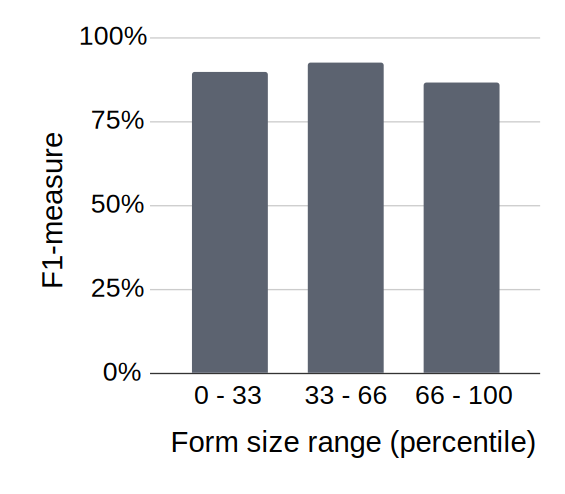
\includegraphics[width=0.45\linewidth,trim=11mm 9mm 7mm 7mm,clip]{accessibility_repair/figures/stratified.pdf}
	\caption{Comparison of labeling inference F1-measure for different form size ranges.}
	\label{fig:stratified}
\end{figure}

\subsubsection{Threats to validity}
In order to avoid any selection bias, 
we chose test subjects (i.e., web sites) 
randomly with the mentioned 
criteria in \Cref{subsec:rq1}. 
The subjects cover diverse categories 
(e.g. news, education, commerce), 
with around two orders of magnitude of 
form sizes, ranging from 17 up to 1552 elements.
This diversity of topics and sizes helps in 
ensuring subjects are representative 
of real-world scenarios, thereby mitigating the 
external validity of the study by making the 
results generalizable.
To make the study replicable and mitigate researcher bias, 
we made available online a link to our tool 
implementation and evaluation data~\cite{tool-and-data}.




% !TEX root =  paper.tex

\subsection{Results and Discussion}\label{sec:discussion}

\begin{figure}[t]
    \centering
    \includegraphics[trim={0.3cm 0.3cm 0.3cm 0.3cm},clip,height=7.9cm, width=0.72\textwidth]{testability/figures/DOM-boxplot.eps}
    \caption{Accuracy of the inferred augmented DOM for each evaluated application in table \ref{table:eval-apps}. A total of 50 canvas elements in five different applications where used for this experiment.}
    \label{fig:result-DOM-accuracy}
\end{figure}

\head{Accuracy}
Figure \ref{fig:result-DOM-accuracy} shows box plots for the accuracy of \tool. 
The x-axis shows our subject applications, and the y-axis shows the  similarity percentage between the original canvas and the canvas regenerated from the inferred augmented canvas DOM. The runtime average for the tool is relatively fast at around 4 $\pm$ 0.3 seconds.

We make a number of observations from Figure \ref{fig:result-DOM-accuracy}. First, we note that most inferred DOMs have an accuracy close to or above $90 \%$ (the average for the dataset is $91.2 \% \pm 1.3$). Furthermore, at the highest and lowest of outliers, the accuracy ranges between $98 \%$ and $85 \%$. Therefore, we conclude from these results that the DOM inference process is relatively accurate in representing the canvas.

As for the accuracy at the lower end of the outliers, the reason for this is the inability of the probabilistic Hough transform used by the algorithm (as described in section \ref{sec:approach}) to generate segments to cover the small boundaries of small objects. These often take the form of small appendages connected to various objects, and the probabilistic Hough transform misses such small appendages. In a future version of the algorithm, we plan to improve the performance by finding a more suitable alternative than the probabilistic transform.

\head{Effectiveness}
Table \ref{tbl:result-fault-injections} shows the effectiveness results for \tool. 
Each row shows the total number of faults injection performed on the application, and then the number of true positives and false negatives reported by \tool, as described in section \ref{sec:experimental-procedure}.

From Table \ref{tbl:result-fault-injections}, we note that the overall rate of detecting true positives is $93\%$ and the overall rate of false negatives is $7\%$. Furthermore, we note that the per-application true positive rate varies from 16 out of 20 ($80\%$, lowest) to 20 out of 20 ($100\%$, highest). 
As such, we conclude from these results that the approach is relatively reliable in detecting faults in canvas elements. 

The main reason for the false negatives is that the probabilistic Hough transform used by the algorithm was unable to generate segments that would cover some of the injected shapes that were small appendages to other objects and this resulted in no modification to the segments set of the object. This is therefore reflected as a false negative. As part of our future improvements, we would like to improve the true positives rate even further by finding a better alternative to the probabilistic transform.

\begin{table}[b]
\setlength{\tabcolsep}{6pt}
\renewcommand{\arraystretch}{0.9}
\centering
\caption{Results of detecting fault injections}
\begin{tabular}{lccc}
\toprule
\textbf{Application} &  \textbf{\# Injections}  &  \textbf{\# True Positives} & \textbf{\# False Negatives} \\
\midrule
JBrowse~\cite{eval_app_jbrowse}      & 20 &  18  &  2 \\
Reactome~\cite{eval_app_reactome}    & 20 &  20  &  0 \\
Scribl~\cite{eval_app_scribl}        & 20 &  16  &  4 \\
Gibberish~\cite{eval_app_gibberish}  & 20 &  19  &  1  \\
iCanplot~\cite{eval_app_icanplot}    & 20 &  20  &  0 \\
\midrule
Total:  & 100   &  $93 \%$ &  $7 \%$ \\

\bottomrule
\end{tabular}
\label{tbl:result-fault-injections}
\end{table}

\head{Threats to Validity}
Our choice of subject applications could be a source of external threat to validity. In order to mitigate this threat, we select subject applications from a wide range of complexity (from around 7,000 to more than 100,000 LOC), and also select the applications from a varying assortment of fields, such as medicine, music, and chemistry. Another related threat is the relatively low number (five) of evaluated subjects. We mitigate this threat by extracting a random collection of 50 canvas snapshots for these applications and running 100 fault injections. \hl{Furthermore, some aspects in the fault injection process could be a source of internal threat to validity. There is currently no compilation of the types of faults that exist for canvases. Accordingly, 
in order to mitigate this threat and have an unbiased fault injection process, we chose to inject random shapes into the canvas. 
We also adopt a uniform approach of consistently injecting random objects on the canvas regardless of the applications's API, as opposed to individually injecting faults by modifying the specific API parameters of each canvas app. This helps in ensuring equally random fault injection across subjects. 
Furthermore, and perhaps most importantly, we do not have access to the objects on the canvas due to the lack of observable state in the canvas, which is the very problem that our approach is trying to solve. Accordingly, due to absence of access to canvas objects, simulating a fault by removing a certain object is not practically achievable.} Another related threat is the possible bias in the determination of true positives or false negatives. We mitigate this threat by injecting faults across all trials and then using a quantitative distance metric with a normalized range to allow a direct binarization of results into true positives and false negatives. 

Another potential threat to validity is the issue of cross-browser compatibility. We note that the rendering of canvas elements is categorically different from rendering regular web pages. When rendering a page, the browser has to continuously maintain a DOM and regularly recompute layout position and visual properties of the page elements before rendering. For canvas, however, the browser does not maintain any layout information about the canvas, and simply paints the pixels from the API call directly on screen. All browsers relay the pixel-by-pixel rendering directly to the canvas. Canvas elements have no observable state and browsers do not participate in maintaining what does or does not get rendered. This is the opposite of rendering webpages.

To the best of our knowledge, there is no evidence in the literature of cross-browser incompatibilities for canvas elements. Furthermore, in a recent study \cite{bajaj2014mining} categorizing questions asked by developers on StackOverflow, canvas related questions were mostly about how to use the canvas API. There was no reported pattern of questions on canvas-related cross browser incompatibility issues. In addition, and more importantly, from our own use and testing of canvas elements, we did not notice incompatibility issues either. For these reasons, we do not consider cross-browser incompatibility to be a threat to the validity of the proposed approach.



% !TEX root =  manuscript.tex
\section{Prior Work}\label{sec:related}

To the best of our knowledge, 
there are no existing surveys or systematic literature reviews that 
share a similar goal to this chapter. 
\hl{
This section discusses  
a broader range of research areas in order to put 
the survey in its proper context.
We therefore begin by discussing secondary studies concerning 
computer vision-based techniques 
in various non-software engineering fields. 
While such studies are not directly related to our topic of discussion, 
they help place the survey within wider context of other similar surveys. 
Second, we explore other surveys that 
are interdisciplinary in nature, 
given the interdisciplinary nature of our survey.
Finally, we discuss visual GUI testing 
techniques, an area with a relatively large 
number of papers employing visual analysis techniques. 
}


\header{Surveys on Computer Vision-based Engineering}
In this subsection, we discuss some of the surveys or systematic literature reviews 
concerning the use of computer vision in various engineering fields. 
We note that these are non-software engineering fields 
(e.g., aerospace or automotive engineering) 
and are included here for the sake of completeness. 

Kumar~\cite{cv-fabric-defect} catalogues the 
fabric defect detection methodologies reported 
in about 150 references into three main categories: 
statistical, spectral and model-based. 
They conclude that despite the significant progress 
in last decade, the problem of fabric defect detection 
still remains challenging and requires effort by 
combining existing approaches. 
%
Kanellakis and Nikolakopoulos~\cite{cv-for-uavs} 
present a comprehensive literature review on vision 
based applications for unmanned aerial vehicles (UAVs) focusing mainly on current 
developments and trends. Computer vision techniques are used 
mainly for visual localization and mapping, 
obstacle detection and avoidance, aerial target 
tracking, and guidance. Among the limitations, 
it is mentioned that the algorithms are based on 
rigid assumptions such as low speed vehicles 
that do not account for fast scene alterations. 
Thus, the main challenge is to design solutions 
that can quickly react to ever changing sceneries, 
characterized by a high degree of dynamism and evolution. 
%
Liu and Dai~\cite{5508131} discuss solutions 
for UAVs from three main families, namely visual 
navigation, aerial surveillance and airborne 
visual simulation.
%
Al-Kaff et al.~\cite{ALKAFF2018447} provide another 
survey of techniques for UAVs, particularly 
visual navigation algorithms, obstacle detection 
and avoidance and aerial decision-making. It is 
mentioned that artificial perception applications 
have represented important advances in the latest 
years in the expert system field related to unmanned aerial vehicles. 

Gandhi and Triveli~\cite{1706871} discuss the recent 
research on pedestrian detection and collision 
prediction. Among the information gathered by 
the various sensors, the camera's image is one 
of the most used, along with visual analysis 
techniques for behaviour modelling in accident 
prediction, direction estimation, and collision prediction. 
%
Brunetti et al.~\cite{BRUNETTI201817} discuss 
vision-based pedestrian detection systems pertaining 
to three different application fields: video 
surveillance, human-machine interaction and 
analysis. Notably, they discuss both the 
differences between 2D and 3D vision systems, 
and indoor and outdoor systems.
%
Janai et al.~\cite{DBLP:journals/corr/JanaiGBG17} 
provides a comprehensive survey on problems, 
datasets, and methods in computer vision for 
autonomous vehicles. First, they overview the 
datasets and benchmarks used in autonomous 
driving research. Then, the discuss the state 
of the art on several relevant topics, 
including recognition, reconstruction, motion 
estimation, tracking, scene understanding, and 
end-to-end learning.

\header{Interdisciplinary Surveys in SE}
Interdisciplinary surveys are often used to collect 
and analyze a body of knowledge across the boundaries 
between two or more fields. 
Here, we discuss some of the 
surveys or systematic literature reviews that have analyzed scientific and social 
fields from a software engineering perspective. 

Zhang et al.~\cite{Zhang-TSE} provide a comprehensive 
survey of techniques for testing machine learning systems. 
The survey covers 144 papers on different 
testing properties such correctness, robustness, 
and fairness, testing components 
(e.g., data, learning program, and frameworks), 
testing workflow (e.g., test generation and 
test evaluation), and application scenarios 
(e.g., autonomous driving, machine translation). 
The paper also analyses trends concerning datasets, 
research trends, and research focus, 
concluding with research challenges and promising 
research directions in machine learning testing.
%
Besz\'{e}des~\cite{Beszdes2019InterdisciplinarySO} 
performed a systematic analysis of fault localization 
literature across different engineering fields, 
with the aim to find solutions in non-software areas 
that could be successfully adapted to software fault 
localization. Among their findings, they indicate that 
some classes of methods in computer networks literature are good 
candidates for adaptation, and could potentially be 
reused for software fault localization. 
%
Van der Linden and Hadar~\cite{8283537} performed a 
systematic literature review of physics of notation applications, 
a conceptual modelling language used for  
requirement specification. They analyzed what 
notations have been evaluated and designed using 
the physics of notation, for what reasons, 
to what degree applications consider requirements 
of their notation's users, and how verifiable these 
applications are. 
%
% Mao et al.~\cite{MAO201757} provide a comprehensive 
% survey of the use of crowdsourcing in software engineering, 
% summarising industrial crowdsourcing practice in software 
% engineering and the corresponding case studies. They 
% further analyzed the software engineering domains, 
% tasks and applications for crowdsourcing and the 
% platforms and stakeholders involved in realizing 
% crowdsourced SE solutions. 

% Similarly to the mentioned works, our survey is also 
% ``approach-oriented'' as it focuses on exploring how 
% approaches from one field (i.e., CV) have been employed 
% in a different field (i.e., SE), for what problems they 
% have been used, and what are the main pros and cons. 
% In contrast, to the best of our knowledge, our treatment 
% of computer vision in software engineering solutions is 
% novel in the software engineering literature, because 
% it comprehensively look at the solutions applied to 
% any stage of the software life cycle. 

Sabaren et al.~\cite{Sabaren-2018-JCST} conduct a systematic 
literature review of cross-browser regression testing.
In their survey, their goal was to collect the 
various techniques that 
have been proposed to perform cross-browser testing. 
The authors also describe several 
challenges in this specific context, such as the 
automatic identification of dynamic components in a 
user interface, which undermines the effectiveness of 
proposed testing techniques, causing many false 
positives in practice.
We note that the survey of~\citet{Sabaren-2018-JCST} has  
found 11 papers that happened to be in our final pool of \numberOfPapers 
collected papers. This is a happenstance since our survey 
has a different objective for the following reasons. 
The work by~\citet{Sabaren-2018-JCST} answers the following
question: what approaches have been used to 
conduct cross-browser regression testing.
In contrast, our work is not concerned at all with that problem. 
Our work answers the following question: in what ways have computer 
vision been used to advance software engineering. 
The reason we had some common papers is because regression testing 
happened to be an area where visual techniques were found 
to be particularly useful. 
However, in terms of the scope and objective, there is no overlap.
%
In other words, \citet{Sabaren-2018-JCST} focus on a specific 
problem (i.e., cross-browser regression testing), regardless 
of what approaches were used (e.g., DOM analysis, 
state space navigation, visual analysis). 
That is, the survey in \citet{Sabaren-2018-JCST} is 
\emph{problem-specific} but approach-agnostic. 
In contrast, our survey is \emph{approach-specific} but 
problem-agnostic. Any overlap between the two surveys is because 
some papers happen to be in the pool of both surveys, 
but not because both surveys perform the same objective or have 
the same research questions. 
We focus on a specific approach 
(i.e., computer vision techniques), but consider its 
potential for any area of software engineering 
(e.g., testing, maintenance, development, design, requirements). 
In summary, none of the aforementioned surveys have a similar 
goal as that of this chapter. 

\header{Visualization Research}
Visualization is the process of creating diagrams, charts, or any other 
kind of representation, from a given dataset. 
Visualization is part of any scientific process regardless of the field, 
and therefore has also been used in software engineering. 
There are a number of surveys on the use of visualization
in various aspects of software engineering,
such as surveys on visualization for software security~\cite{wagner2015survey,zhang2012survey},
surveys on visualization for static analysis~\cite{caserta2010visualization},
development coordination~\cite{storey2005use},
maintenance and evolution~\cite{novais2013software, koschke2003software},
to name a few. 
Visualization, however, is not the scope of this survey. 

\header{Visual GUI Testing}
Issa et al~\cite{6320526} first introduced the notion of
\textit{visual testing} as a subset of traditional GUI testing.
In their analysis, the authors conducted a study of bugs
in four open source systems, and found that visual bugs
represent between 16\% and 33\% of reported defects in those systems. 
In recent years, researchers and practitioners have started
conducting empirical experiments aiming at understanding the
comparative performance of a few visual testing approaches. 
For instance, Al\'{e}groth et al.~\cite{alegroth2017,
alegroth2015conceptualization}
present a case study of the benefits and challenges of
using visual GUI testing by the team at one software company. 
In another study, Al\'{e}groth et al.~\cite{8367046} study 
the applicability and feasibility of Visual GUI testing in 
an industrial Continuous Integration environment, describing the 
main challenges faced by researchers to make it effective in practice. 
Garousi et al.~\cite{garousi2017comparing} compare two popular visual
testing tools (Sikuli and JAutomate) in one industrial project,
and go through differences in test creation process, execution,
and maintenance.

All such works analyze different technical and social aspects 
related to the use of Visual GUI testing in a specific context 
(i.e., the development and maintenance of test code). 
In contrast, our work is agnostic to any specific area or context. 
That is, it does not aim to focus on GUI testing. 
Rather, the goal is to broadly examine the use of visual techniques 
across any software engineering area (e.g., requirements, design, 
development, testing, maintenance) and for any task (e.g., refactoring, 
reverse engineering, regression testing). 


\begin{figure*}
    \centering
    %\fbox{
    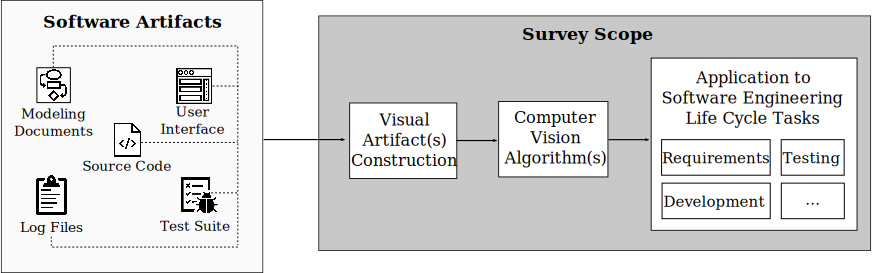
\includegraphics[scale=0.50]{survey/figures/scope-horizontal}
    %}
    \caption{Overview of the scope of this survey.}
    \label{fig:scope}
\end{figure*}





%\section{Future Work}\label{sec:future}

In our future work we intend to
\section{Conclusions}
\label{sec:conclusions}

Web applications based on canvas elements allow the creation of dynamic graphics, interactive user interfaces, and scalable visualizations. However, there has been little to no research in literature in terms of testing canvas elements. This chapter proposed a testing approach, implemented in a tool, \tool, based on visual analysis of the screenshot of canvas elements, and generating an augmented DOM tree for the canvas element to allow making test assertions on it. We evaluated the accuracy of the proposed approach and its effectiveness in detecting faults injected in canvas elements. We found the inference process to be relatively accurate (around $91\%$ accuracy on average) with a true positive rate of $93\%$ in detecting fault injections. 
We note, however, that the goal of this work is to provide developers with the fundamental capability of observing the canvas state and making assertions on it. However, it does not provide a complete testing solution, but rather make it \emph{possible} to perform the testing process itself, thereby improving testability. As part of future work, a more through canvas testing solution can be provided such that it will cover more complex and resizable canvas elements, and generate the tests in a fashion that developers might prefer (e.g., using relative positioning in assertions). 
% conference papers do not normally have an appendix

% use section* for acknowledgement
%\section*{Acknowledgment}
%
%
%The authors would like to thank...
%more thanks here

% trigger a \newpage just before the given reference
% number - used to balance the columns on the last page
% adjust value as needed - may need to be readjusted if
% the document is modified later
%\IEEEtriggeratref{8}
% The "triggered" command can be changed if desired:
%\IEEEtriggercmd{\enlargethispage{-5in}}

% references section

% can use a bibliography generated by BibTeX as a .bbl file
% BibTeX documentation can be easily obtained at:
% http://www.ctan.org/tex-archive/biblio/bibtex/contrib/doc/
% The IEEEtran BibTeX style support page is at:
% http://www.michaelshell.org/tex/ieeetran/bibtex/
%\bibliographystyle{IEEEtran}
% argument is your BibTeX string definitions and bibliography database(s)
%\bibliography{IEEEabrv,../bib/paper}
%
% <OR> manually copy in the resultant .bbl file
% set second argument of \begin to the number of references
% (used to reserve space for the reference number labels box)
%\begin{thebibliography}{1}

%\bibitem{IEEEhowto:kopka}
%H.~Kopka and P.~W. Daly, \emph{A Guide to \LaTeX}, 3rd~ed.\hskip 1em plus
%  0.5em minus 0.4em\relax Harlow, England: Addison-Wesley, 1999.
%\bibliography{IEEEabrv,bibliography.bib}
\balance
\bibliography{bibliography.bib}
\balance
\bibliographystyle{IEEEtran}

%\end{thebibliography}




% that's all folks
\end{document}


